%%% DOCUMENT TYPE %%%%%%%%%%%%%%%%%%%%%%%%%%%%%%%%%%%%%%%%%%%%%%%%%%%%%%%%%%%%%%



%%% SETUP %%%%%%%%%%%%%%%%%%%%%%%%%%%%%%%%%%%%%%%%%%%%%%%%%%%%%%%%%%%%%%%%%%%%%%

%%% DOCUMENT TYPE %%%%%%%%%%%%%%%%%%%%%%%%%%%%%%%%%%%%%%%%%%%%%%%%%%%%%%%%%%%%%%

\documentclass[9pt, a4paper, twocolumn, landscape]{extarticle}

%%% PACKAGES %%%%%%%%%%%%%%%%%%%%%%%%%%%%%%%%%%%%%%%%%%%%%%%%%%%%%%%%%%%%%%%%%%%

% Encoding

\usepackage[utf8]{inputenc}
\usepackage[T1]{fontenc}

% Geometry

\usepackage{geometry} % edit margins of paper
\usepackage{setspace} % edit line spacing
\usepackage{fancyhdr} % header, footer
\usepackage{titlesec} % edit format of titles

% Visual

\usepackage[dvipsnames]{xcolor} % colors
\usepackage{tikz} % graphics
\usepackage[framemethod=tikz]{mdframed} % frames, better theorems

% Math

\usepackage{amsmath} % math tools
\usepackage{amssymb} % math symbols
\usepackage{amsthm} % thereoms
\usepackage{mathtools} % math tools

% Referencing

\usepackage{nameref}
\usepackage{hyperref}
\usepackage{cleveref}

% Useful

\usepackage[shortlabels]{enumitem} % enumerations

% Other

\usepackage{lastpage} % get number of last page
\usepackage{physics}
\usepackage{bbm}

%%% MARGINS %%%%%%%%%%%%%%%%%%%%%%%%%%%%%%%%%%%%%%%%%%%%%%%%%%%%%%%%%%%%%%%%%%%%

\geometry{a4paper, landscape, left=10mm, right=10mm, top=10mm, bottom=10mm, includehead}

%%% COLORS %%%%%%%%%%%%%%%%%%%%%%%%%%%%%%%%%%%%%%%%%%%%%%%%%%%%%%%%%%%%%%%%%%%%%

%%% TITLES %%%%%%%%%%%%%%%%%%%%%%%%%%%%%%%%%%%%%%%%%%%%%%%%%%%%%%%%%%%%%%%%%%%%%

\colorlet{color-section}                {Blue}
\colorlet{color-subsection}             {RoyalPurple}
\colorlet{color-paragraph}             {MidnightBlue}
\colorlet{color-subsubsection}	{CadetBlue}
%%% MATH BOXES %%%%%%%%%%%%%%%%%%%%%%%%%%%%%%%%%%%%%%%%%%%%%%%%%%%%%%%%%%%%%%%%%

\colorlet{color-definition}              {Blue!20}%{SpringGreen!20}
\colorlet{color-theorem}                {Brown!25}%{Apricot!13}
\colorlet{color-proposition}            {ProcessBlue!13}% {Apricot!13}
\colorlet{color-corollary}              {Salmon!12}%{Apricot!13}
\colorlet{color-lemma}                  {Brown!7}%{Apricot!13}
\colorlet{color-remark}                 {Gray!4}
\colorlet{color-example}                {Lavender!7}
% \colorlet{color-proof}                  {FILL COLOR HERE}


%%% CAPTIONS %%%%%%%%%%%%%%%%%%%%%%%%%%%%%%%%%%%%%%%%%%%%%%%%%%%%%%%%%%%%%%%%%%%

%%% CAPTION DEFINITION %%%%%%%%%%%%%%%%%%%%%%%%%%%%%%%%%%%%%%%%%%%%%%%%%%%%%%%%%

\newcommand*{\definitionname}{Definition}
\newcommand*{\theoremname}{Theorem}
\newcommand*{\propositionname}{Proposition}
\newcommand*{\corollaryname}{Corollary}
\newcommand*{\lemmaname}{Lemma}
\newcommand*{\remarkname}{Remark}
\newcommand*{\examplename}{Example}


%%% SHORTCUTS %%%%%%%%%%%%%%%%%%%%%%%%%%%%%%%%%%%%%%%%%%%%%%%%%%%%%%%%%%%%%%%%%%

%%% SINGLE SYMBOLS %%%%%%%%%%%%%%%%%%%%%%%%%%%%%%%%%%%%%%%%%%%%%%%%%%%%%%%%%%%%

% Logic

% \forall exists
% \exists exists
% \lnot exists
% \lor exists
% \land exists
\newcommand*{\limp}{\rightarrow}
\newcommand*{\limps}{\; \limp \;} % \limp with some space around
\newcommand*{\leqv}{\leftrightarrow}
\newcommand*{\leqvs}{\; \leqvs \;} % \leqv with some space around

% Meta Logic

% \implies exists
% \iff exists

% Colon Stuff

\newcommand*{\cl}{\colon}
\newcommand*{\cleq}{\coloneqq}
\newcommand*{\eqcl}{\eqqcolon}

% Sets

\newcommand*{\N}{\mathbb{N}} % natural numbers
\newcommand*{\Z}{\mathbb{Z}} % integers
\newcommand*{\Q}{\mathbb{Q}} % rational numbers
\newcommand*{\R}{\mathbb{R}} % real numbers
\newcommand*{\C}{\mathbb{C}} % complex numbers

%%% MATH OPERATORS %%%%%%%%%%%%%%%%%%%%%%%%%%%%%%%%%%%%%%%%%%%%%%%%%%%%%%%%%%%%%

% General

\DeclareMathOperator{\id}{id}
\DeclareMathOperator{\sgn}{sgn}
\DeclareMathOperator{\vol}{vol}
\DeclareMathOperator{\supp}{supp}
\let\grad\relax
\DeclareMathOperator{\grad}{grad}
\DeclareMathOperator{\rot}{rot}
\let\div\relax
\DeclareMathOperator{\div}{div}
%%% TEMPLATES %%%%%%%%%%%%%%%%%%%%%%%%%%%%%%%%%%%%%%%%%%%%%%%%%%%%%%%%%%%%%%%%%%

% General

% write a set definition like: { #1 | #2 }
\newcommand*{\setdefinition}[2]{
  \{#1 \mid #2\}
}

% write a nice map definition
\newcommand*{\mapdefinition}[5]{
  \begin{align*}
    #1 \cl #2 &\to     #3 \\
           #4 &\mapsto #5
  \end{align*}
}


%%% FORMATTING %%%%%%%%%%%%%%%%%%%%%%%%%%%%%%%%%%%%%%%%%%%%%%%%%%%%%%%%%%%%%%%%%

%%% HEADER, FOOTER %%%%%%%%%%%%%%%%%%%%%%%%%%%%%%%%%%%%%%%%%%%%%%%%%%%%%%%%%%%%%

\pagestyle{fancy}
\fancyhf{} % clear everything
\lhead{}
\chead{\bfseries Quantum Physics}
\rhead{Seite \thepage / \pageref*{LastPage}}
\lfoot{}
\cfoot{}
\rfoot{}

%%% TITLE FORMAT %%%%%%%%%%%%%%%%%%%%%%%%%%%%%%%%%%%%%%%%%%%%%%%%%%%%%%%%%%%%%%%

\setcounter{secnumdepth}{2}

\titleformat{\chapter}[display]
{\normalfont\huge\bfseries}{\chaptertitlename\ \thechapter}{20pt}{\Huge}
\titleformat{\section}[frame]
{\normalfont\LARGE\bfseries\color{color-section}\scshape\filright}{\thesection}{1ex}{\filcenter}
\titleformat{\subsection}
{\normalfont\large\bfseries\color{color-subsection}}{\thesubsection}{1em}{}
\titleformat{\subsubsection}
{\normalfont\normalsize\bfseries\color{color-subsubsection}}{\thesubsubsection}{1em}{}
\titleformat{\paragraph}[runin]
{\normalfont\normalsize\bfseries\color{color-paragraph}}{\theparagraph}{1em}{}
\titleformat{\subparagraph}[runin]
{\normalfont\normalsize\bfseries}{\thesubparagraph}{1em}{}

%%% SPACING %%%%%%%%%%%%%%%%%%%%%%%%%%%%%%%%%%%%%%%%%%%%%%%%%%%%%%%%%%%%%%

% Titles

\titlespacing*{\chapter}{0pt}{50pt}{40pt}
\titlespacing*{\section}{0pt}{3.5ex plus 1ex minus .2ex}{2.3ex plus .2ex}
\titlespacing*{\subsection}{0pt}{3.25ex plus 1ex minus .2ex}{1.5ex plus .2ex}
\titlespacing*{\subsubsection}{0pt}{3.25ex plus 1ex minus .2ex}{1.5ex plus .2ex}
\titlespacing*{\paragraph}{0pt}{1.25ex plus 1ex minus .2ex}{1em}
\titlespacing*{\subparagraph}{\parindent}{3.25ex plus 1ex minus .2ex}{1em}

% Text, Paragraphs

%\setstretch{1.05} % scaling of space between lines
%\setlength{\parindent}{0pt} % indentation of paragraphs
%\setlength{\parskip}{4.0pt plus 1.0pt minus 1.0pt} % space between paragraphs
\setlength{\parskip}{0pt}

%%% SYMBOLS USED BY NUMBERINGS, ENVIRONMENTS, ... %%%%%%%%%%%%%%%%%%%%%%%%%%%%%%

% \renewcommand*\qedsymbol{$\blacksquare$} % alternative QED symbol
\renewcommand{\thefootnote}{\arabic{footnote}} % normal footnotes on page
\renewcommand{\thempfootnote}{\fnsymbol{mpfootnote}} % footnotes on minipages, e.g. in mdframed environments

%%% LISTS, ENUMERATIONS %%%%%%%%%%%%%%%%%%%%%%%%%%%%%%%%%%%%%%%%%%%%%%%%%%%%%%%%

% 'itemize'

\setlist[itemize]{noitemsep, topsep=0pt}

% 'enumerate'

% no special settings at the moment

% 'description'

% no special settings at the moment

% 'axioms'

\newlist{axioms}{enumerate}{2}
\setlist[axioms]{itemsep=0pt,label*=\arabic*.}

%%% MDFRAMED PATCH %%%%%%%%%%%%%%%%%%%%%%%%%%%%%%%%%%%%%%%%%%%%%%%%%%%%%%%%%%%%%

\usepackage{xpatch}

\makeatletter
\xpatchcmd{\endmdframed}
  {\aftergroup\endmdf@trivlist\color@endgroup}
  {\endmdf@trivlist\color@endgroup\@doendpe}
  {}{}
\makeatother

%%% MDFRAMED STYLES %%%%%%%%%%%%%%%%%%%%%%%%%%%%%%%%%%%%%%%%%%%%%%%%%%%%%%%%%%%%

% thick frame and bar for title

\mdfdefinestyle{style-box}{
  skipabove=1.5ex plus .5ex minus .2ex,
  skipbelow=1ex plus .2ex minus .2ex,
  linewidth=2pt,
  linecolor=Gray!20,
%   roundcorner=3pt,
  innerleftmargin=0.5\baselineskip,
  innerrightmargin=0.5\baselineskip,
  innertopmargin=0.4\baselineskip,
  innerbottommargin=0.4\baselineskip,
  frametitlebackgroundcolor=Gray!20,
  frametitleaboveskip=0.3pt,
  frametitlebelowskip=0.3pt,
  theoremseparator=,
  theoremspace=\hfill,
  theoremtitlefont=\mdseries\scshape,
  nobreak=true
}

% highlighted background

\mdfdefinestyle{style-background}{
  skipabove=1.5ex plus .5ex minus .2ex,
  skipbelow=1ex plus .2ex minus .2ex,
  hidealllines=true,
  backgroundcolor=Gray!5,
  innerleftmargin=0.5\baselineskip,
  innerrightmargin=0.5\baselineskip,
  innertopmargin=0.4\baselineskip,
  innerbottommargin=0.4\baselineskip,
}

% thin frame

\mdfdefinestyle{style-leftline}{
  skipabove=1.5ex plus .5ex minus .2ex,
  skipbelow=1ex plus .2ex minus .2ex,
  linewidth=1pt,
  linecolor=Gray!50,
  topline=false,
  bottomline=false,
  rightline=false,
  innerleftmargin=0.5\baselineskip,
  innerrightmargin=0,
  innertopmargin=0.2\baselineskip,
  innerbottommargin=0.0\baselineskip,
}

%%% ENVIRONMENTS %%%%%%%%%%%%%%%%%%%%%%%%%%%%%%%%%%%%%%%%%%%%%%%%%%%%%%%%%%%%%%%

% Definition

\mdtheorem[
  style=style-box,
  linecolor=color-definition,
  frametitlebackgroundcolor=color-definition
]{definition}{\definitionname}[section]

% Theorem

\mdtheorem[
  style=style-box,
  linecolor=color-theorem,
  frametitlebackgroundcolor=color-theorem,
  font=\itshape
]{theorem}{\theoremname}[section]

% Proposition

\mdtheorem[
  style=style-box,
  linecolor=color-proposition,
  frametitlebackgroundcolor=color-proposition,
  font=\itshape
]{proposition}[theorem]{\propositionname}

% Corollary

\mdtheorem[
  style=style-box,
  linecolor=color-corollary,
  frametitlebackgroundcolor=color-corollary,
  font=\itshape
]{corollary}[theorem]{\corollaryname}

% Lemma

\mdtheorem[
  style=style-box,
  linecolor=color-lemma,
  frametitlebackgroundcolor=color-lemma,
  font=\itshape
]{lemma}[theorem]{\lemmaname}

\theoremstyle{remark}

% Remark

\newtheorem*{remark}{\remarkname}
\surroundwithmdframed[
  style=style-background,
  backgroundcolor=color-remark
]{remark}

% Example

\newtheorem*{example}{\examplename}
\surroundwithmdframed[
  style=style-background,
  backgroundcolor=color-example
]{example}

% Proof

\surroundwithmdframed[
  style=style-leftline
]{proof}

%%% TEXT FORMATTING %%%%%%%%%%%%%%%%%%%%%%%%%%%%%%%%%%%%%%%%%%%%%%%%%%%%%%%%%%%%

% definitions
\let\epsilon\varepsilon
\renewcommand\emptyset{\varnothing}
\newcommand*{\df}[1]{\colorbox{color-definition}{\emph{#1}}}


%%% LANGUAGE %%%%%%%%%%%%%%%%%%%%%%%%%%%%%%%%%%%%%%%%%%%%%%%%%%%%%%%%%%%%%%%%%%%

%%% SETUP %%%%%%%%%%%%%%%%%%%%%%%%%%%%%%%%%%%%%%%%%%%%%%%%%%%%%%%%%%%%%%%%%%%%%%

\usepackage[english]{babel}

%%% CAPTION REDEFINITION %%%%%%%%%%%%%%%%%%%%%%%%%%%%%%%%%%%%%%%%%%%%%%%%%%%%%%%



%%% HYPHENATION %%%%%%%%%%%%%%%%%%%%%%%%%%%%%%%%%%%%%%%%%%%%%%%%%%%%%%%%%%%%%%%%


\usepackage[arrow, matrix, curve]{xy}
\usepackage{wrapfig}
\usepackage{bm}
\usepackage{multicol}
\usepackage{xcolor}
\usepackage{mathrsfs} 
\usepackage{bbm}
\renewcommand\vec{\boldsymbol}

%%% DOCUMENT %%%%%%%%%%%%%%%%%%%%%%%%%%%%%%%%%%%%%%%%%%%%%%%%%%%%%%%%%%%%%%%%%%%

\begin{document}

\section{Stuff dump}

\paragraph{Cambell Baker Hausdorf} Für alle $t \in \mathbb{R}$ 
$$ 
\exp(t A) \exp(t B)= \exp \left(t A+t B+\frac{t^2}{2}[A, B]
+\frac{t^3}{12} [A,[A, B]] +\frac{t^3}{12}[B,[B, A]]+\mathscr{O}\left(t^4\right)\right)
$$

\paragraph{Creation-/Annihilation Operators}in second quantisation:
$$\left[\hat{a}_i^*, \hat{a}_j^*\right]=0, \quad\left[\hat{a}_i, \hat{a}_j\right]=0, \quad\left[\hat{a}_i, \hat{a}_j^*\right]=\delta_{i, j} \hat{\mathrm{id}}$$


\paragraph{Bernoulli Trial} Probability of $k$ successes in a bernoulli experiment $B(n,p)$:
$$P(k)=\left(\begin{array}{l}
  n \\
  k
  \end{array}\right) p^k q^{n-k} $$

\paragraph{Bayes' rule}  $$
\operatorname{Pr}[A \mid B \wedge C]=\frac{\operatorname{Pr}[B \mid A \wedge C]}{\operatorname{Pr}[B \mid C]} \operatorname{Pr}[A \mid C]
$$

\paragraph{Maxwell equations} we have \\
$ \nabla E = \frac{\rho}{\epsilon_0}  \quad  $  \ (Gauss law)   \\
$ \nabla B = 0 $ \\
$ \nabla \times E = \ - \frac{\partial B}{\partial t} \quad  $ \  (Faraday's law of induction) \\
$ \nabla \times B = \frac{1}{c^2} \frac{ \partial E}{\partial t} + \mu_0 J + \epsilon_0 \frac{\partial P} {\partial t} \quad $ \ (Ampere's law)

\paragraph{Delta distribution}
\begin{itemize}
  \item $\int d x e^{i k \cdot x}=(2 \pi) \delta(k)$
  \item $\int_{-\infty}^{+\infty} d x \delta(g(x))=\sum_i \frac{1}{\left|g^{\prime}\left(x_i\right)\right|} $
\end{itemize}

\paragraph{Displacement operator} $D(\eta)=e^{\eta a^{\dagger}-\eta^* a}$

%%% Math stuff dump 

\paragraph{Fourier transform } For $\varphi \in \mathscr{S}\left(\mathbb{R}^n\right)$:\\
(i) $\left(\partial_j \varphi\right)^{\wedge}(k)=i k_j \hat{\varphi}(k)$\\
(ii) $\partial_j \hat{\varphi}(k)=\frac{\partial}{\partial k_j} \hat{\varphi}(k)=\left(-i x_j \varphi\right)^{\wedge}(k)$\\
(iii) $\left(\partial_j \varphi\right)^{\vee}(k)=-i k_j \check{\varphi}(k)$\\
(iv) $\partial_j \check{\varphi}(k)=\left(i x_j \varphi\right)^{\vee}(k)$\\
(v) $\mathcal{F}_x\left[e^{-a x^2}\right](k)=\sqrt{\frac{\pi}{a}} e^{-k^2 a} \quad $ Normalsation 1; osc factor 1

\paragraph{Fundamental Theorem of calculus} $f\left(t_2\right)=f\left(t_1\right)+\int_{t_1}^{t_2} d t \partial_t f(t)$

\paragraph{Normal Distribution} $f(x)=\frac{1}{\sigma \sqrt{2 \pi}} e^{-\frac{1}{2}\left(\frac{x-\mu}{\sigma}\right)^2}$

\paragraph{Residue Theorem} $\oint_{\mathcal{C}} \mathrm{d} z f(z)=\pm 2 \pi i \sum_n \operatorname{Res}\left(z_n\right) \quad $,
$\operatorname{Res}\left(z_n\right)=\lim _{z \rightarrow z_n}\left(z-z_n\right) f(z)$

%%%%%%%%%%%%%%%%%%%%%%%%%%%%%%%%%%%%%%%%%%%%%%%%%%%%%%%%%%%%%%%%%%%%%%%  Quantum mechanics I & II %%%%%%%%%%%%%%%%%%%%%%%%%%%%%%%%%%%%%%%%%%%%%%%%%%%%%%%%%%%%%%%%%%%%%%%%%%%%%%%
\section{Quantum Mechanics I \& II}

\paragraph{Total angular momentum} commutation relations: $\left[\hat{J}_z, \hat{J}_{\pm}\right]=\pm \hat{J}_{\pm}, \quad\left[\hat{J}_{+}, \hat{J}_{-}\right]=2 \hat{J}_z$

\paragraph{Propagator} characterised through \\
(i) $U(t, t)=\mathbf{I}$.\\
(ii) additivity/ unitary: $U(t, s) U(s, r)=U(t, r)$.\\
(iii) The operator $U(t, s)$ satisfies the differential equation
$$
i \hbar \partial_t U(t, s)=H U(t, s)
$$
For $H$ time independent: $U(t, s)=\exp \left(-i H \frac{(t-s)}{\hbar}\right)$\\
General: $U(t, s)=\mathcal{T} \exp \left[-\frac{i}{\hbar} \int_s^t d t^{\prime} H\left(t^{\prime}\right)\right]$. 
If $[H(t),H(s)]=0 \ \forall t,s$ we can omit the time order operator $\mathcal{T}$.

\paragraph{Heisenberg picture} Time dependecy is shifted from states to operators:\\
$$\Psi_H= \Psi(t_0) = U\left(t_0, t\right) \Psi_S(t) \quad \quad A_H=U\left(t_0, t\right) A_S U\left(t, t_0\right)$$
The equation of motion in the Heisenberg picture: 
$$i \hbar \frac{d}{d t} A_H(t) = \left[A_H, H_H\right]+i \hbar \partial_t A_H$$
For $\partial_t H=0$ we have $H_H=H_S$ and $A_H(t)=e^{i H\left(t-t_0\right) / \hbar} A e^{-i H\left(t-t_0\right) / \hbar}$\\
\emph{The Heisenberg picture shows the similaritiy to classical mechanics where we have $\frac{d A}{d t}=\{A, H\}+\partial_t A$.
Replacing the Poisson braket with commutators and imposing the canonical commutator relations gives rise to qunatisation. }

\paragraph{Interaction (Dirac) picture} For $H=H_0+H^{\prime}(t)$. Idea is to shift (trivial) time dependence
of states originating from $H_0$ on to operators: $\Psi_D(t)=U_D\left(t, t_0\right) \Psi_S\left(t_0\right) $ with 
$U_D\left(t, t_0\right)=U_0\left(t_0, t\right) U\left(t, t_0\right)$ where $U$ is the Propagator for $H=H_0 +H'$.\\
For operators $A_D(t)=U_0\left(t_0, t\right) A U_0\left(t, t_0\right)$. We have 
$$i \hbar \partial_t U_D = H_D^{\prime} U_D$$
So in the dirac picture we have the Hamiltonian: $H_D=U H U^{\dagger}+\left(i \partial_t U\right) U^{\dagger} = U H' U^{\dagger} $

\subsection{Light Matter Interaction}

\paragraph{Energy of electromagnetic field} including charges $H=\int \mathrm{d}^3 x \frac{1}{4 \pi}\left(\frac{1}{2}|\vec{E}|^2+\frac{1}{2}|\vec{B}|^2-\phi \vec{\nabla} \cdot \vec{E}\right)$

\paragraph{Electromagetic field in vacuum} ED described by $\vec{\nabla} \cdot \vec{A}=0  \text { and } \square \vec{A}=0$. General solution 
$$\vec{A}(\vec{x}, t)=\frac{1}{\sqrt{L^3}} \sum_{\vec{k}, \lambda}\left[a(\vec{k}, \lambda) \vec{e}(\vec{k}, \lambda) \mathrm{e}^{\mathrm{i}\left(\vec{k} \cdot \vec{x}-\omega_k t\right)}+a^*(\vec{k}, \lambda) \vec{e}^*(\vec{k}, \lambda) \mathrm{e}^{-\mathrm{i}\left(\vec{k} \cdot \vec{x}-\omega_k t\right)}\right]$$
with $a(\vec{k},\lambda)$ amplitudes, $\lambda \in\{1,2\}$ polarisations, $\vec{e}$ polarisation vectors. 

\paragraph{Particle current density} $\hat{\vec{\jmath}}(\vec{x}):=\frac{1}{2 m}(\hat{\vec{p}} \delta(\vec{x}-\hat{\vec{x}})+\delta(\vec{x}-\hat{\vec{x}}) \hat{\vec{p}}) $

\paragraph{Hamiltonian of test particle in Electronmagnetic field} $\hat{H}=\frac{1}{2 m}\left(\hat{\vec{p}}-\frac{q}{c} \vec{A}(\hat{\vec{x}}, t)\right)^2+q \phi(\hat{\vec{x}}, t)+U(\hat{\vec{x}} )$.
Found by guessing the right Lagrangian with Euler-Lagrange equations that yield Newtons law with $\vec{F}=q(\vec{E}+\vec{v} \times \vec{B})$.

\paragraph{Fermis Golden Rule} For Pertubation Hamiltonians of the form $\hat{H}_I(t)=\hat{V} \theta\left(t-t_0\right) \mathrm{e}^{-\mathrm{i} \omega t}+\hat{V}^* \theta\left(t-t_0\right) \mathrm{e}^{\mathrm{i} \omega t}$
we have $$\Gamma_{i \rightarrow f}=\frac{2 \pi}{\hbar}|\langle f|\hat{V}| i\rangle|^2 \delta\left(E_f-E_i-\hbar \omega\right)+\frac{2 \pi}{\hbar}\left|\left\langle f\left|\hat{V}^*\right| i\right\rangle\right|^2 \delta\left(E_f-E_i+\hbar \omega\right)$$\\
The trannsition rate $\Gamma_{i \rightarrow f}$ is the expected number of transitions $\ket*{i} \rightarrow \ket*{f}$ per unit time per particle in state $\ket*{t}$. 

\paragraph{Generators of SO(3)} States transform under SO(3) rotations $|\varphi\rangle \stackrel{R}{\rightarrow} U(R)|\varphi\rangle$. Every SO(3) representation can be written as $U(R(n, \theta))=\exp (-\mathrm{i} \theta \vec{n} \cdot \hat{\vec{J}})$\\
$ \hat{\vec{J}}$ is the vector of generators for the representation (\emph{Angular momentum operator}). Conversely $\hat{\vec{J}}$ determines the representation.\\
Since vector operators should transform under rotations like vectors, we get following condition from general state rotations: $U(R)^* \hat{V}_k U(R) \stackrel{!}{=} \sum_l R_{k l} \hat{V}_l$


%%%%%%%%%%%%%%%%%%%%%%%%%%%%%%%%%%%%%%%%%%%%%%%%%%%%%%%%%%%%%%%%%%%%%%%%%%%%%%% QIT %%%%%%%%%%%%%%%%%%%%%%%%%%%%%%%%%%%%%%%%%%%%%%%%%%%%%%%%%%%%%%%%%%%%%%%%%%%%%%%
%%%%%%%%%%%%%%%%%%%%%%%%%%%%%%%%%%%%%%%%%%%%%%%%%%%%%%%%%%%%%%%%%%%%%%%%%%%%%%% QIT %%%%%%%%%%%%%%%%%%%%%%%%%%%%%%%%%%%%%%%%%%%%%%%%%%%%%%%%%%%%%%%%%%%%%%%%%%%%%%%
%%%%%%%%%%%%%%%%%%%%%%%%%%%%%%%%%%%%%%%%%%%%%%%%%%%%%%%%%%%%%%%%%%%%%%%%%%%%%%% QIT %%%%%%%%%%%%%%%%%%%%%%%%%%%%%%%%%%%%%%%%%%%%%%%%%%%%%%%%%%%%%%%%%%%%%%%%%%%%%%%

\section{Quantum Information Theory}
\paragraph{Quantum probability}
$Pr_\rho[\Lambda] = \Trace{\Lambda \rho} $\\
probabity density: $\quad \rho \in \operatorname{Lin}(\mathcal{H}), \quad \rho \geq 0, \quad \Trace[p] =1$\\
effect / measuremnt: $\Lambda \in \operatorname{Lin}(\mathcal{H}), \quad \Lambda \geq 0, \quad \Lambda \leq \mathbb{I}$ \\

positivity of operators: $S \geq 0$ if $\langle v|S| v\rangle \geq 0 \text { for all } v \in \mathcal{H}$

\paragraph{POVM: postive operator valued measure} set of effects $\{ \Lambda (x)\}^n_{x=1}$ such that
$\Lambda(x) \in \operatorname{Lin}(\mathcal{H}) : \Lambda(x) \geq 0 \ \forall x, \ \sum_x \Lambda(x) =$ $1$

\paragraph{Trace (abstract)} $\Trace{\ketbra*{\Phi}{\Psi}} := \braket*{\Psi}{\Phi}$, then extend linearly. We have cyclidicity
$\Trace[ABC]= \Trace[CAB]$. For basis transformations $\Tr[U \rho U^* ]= \Tr[\rho]$.\\

\paragraph{Bloch sphere}
\begin{multicols}{2}
  Parametisation of states in the spin-($1/2$) picture with Bloch sphere: $|\psi\rangle=\cos \frac{\theta}{2}|0\rangle+e^{i \varphi} \sin \frac{\theta}{2}|1\rangle$.
  Equivalently states can be labled by Bloch- vectors $\hat{n}(\theta, \phi) =\hat{x} \sin \theta \cos \varphi+ \hat{y} \sin \theta \sin \varphi+\hat{z} \cos \theta$ 
  on unit sphere with $\theta \in (0, \pi)$, $\phi \in (0,2 \pi)$. For $- \hat{n}$ we have $(\theta, \phi) \to (\pi - \theta , \phi + \pi) $. And $|\hat{n}\rangle \text { and }|-\hat{n}\rangle $
  are orthogonal.\\
  Every quibit probability density can be written as $\rho=\frac{1}{2}(\mathbb{I}+\vec{r} \cdot \vec{\sigma})$
  where $\vec{r}$ is the Bloch vector with $\norm{\vec{r}} \leq 1$.
    \hspace*{2.5cm} 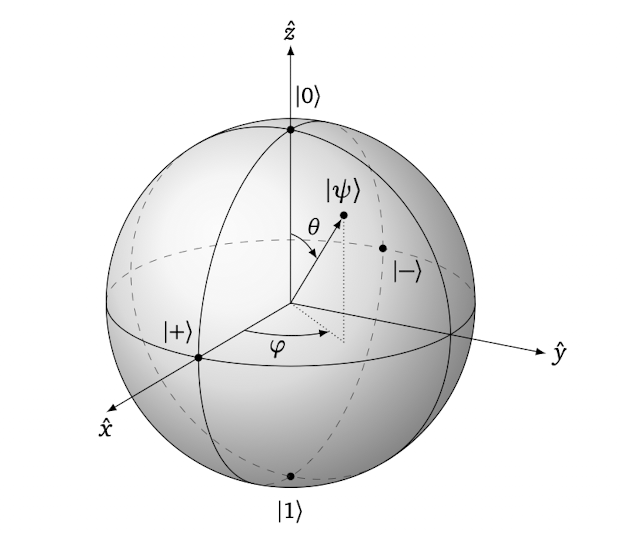
\includegraphics[scale=0.35]{fig/BlochSph.png}
\end{multicols}

\paragraph{pure and mixed states} Projection operators $\ketbra{\Psi}{\Psi}$ assigned to wavefuctions (Norm=1) are pure states. Extreme points of a set of 
states are necessarly pure. States that are not pure are called mixed. 

\subsection{Composite Systems} 
$\mathcal{H}_{AB} = \mathcal{H}_A \otimes \mathcal{H}_B$\\
$\ket{+}_A\otimes \ket{+}_B = \ket*{++}_{AB} = \frac{1}{2} (\ket*{00}_{AB}+ \ket*{01}_{AB}+ \ket*{10}_{AB}+\ket*{11}_{AB})$\\
product state: $\ket{\Psi}\otimes \ket*{\phi} = \ket*{\Psi}_{AB}. \quad$ 
Seprable state is mixture of product states: $\sigma_{A B}=\sum_{k=1}^n P(k) \rho_A(k) \otimes \varphi_B(k). \quad$
Entagled state: $\ket*{\Psi}_{AB}$ such that it cannot be written as seprable state. Pure states are entangled iff their partial states are not pure.\\
Partial trace $\Tr_{AB}[M_{AB}] = \Tr_A[\Tr_B[M_{AB}]]$

\paragraph{Post measurement state} $\rho_{p o s t}^{(i)}=\frac{\Lambda_i \rho \Lambda_i}{\operatorname{tr}\left(\Lambda_i \rho\right)}$

\paragraph{Technical stuff}
\begin{itemize}
  \item Pauli operators: $\begin{array}{l}
    \sigma_x= \quad |0\rangle\langle 1|+| 1\rangle\langle 0| \simeq \ \left(\begin{array}{cc}
    0 & 1 \\
    1 & 0
    \end{array}\right) \\
    \sigma_y=-i|0\rangle\langle 1|+i| 1\rangle\langle 0| \simeq\left(\begin{array}{cc}
    0 & -i \\
    i & 0
    \end{array}\right), \\
    \sigma_z= \quad |0\rangle\langle 0|-| 1\rangle\langle 1| \simeq \ \left(\begin{array}{cc}
    1 & 0 \\
    0 & -1
    \end{array}\right)
    \end{array}$
  \item $\left[\sigma_i, \sigma_j\right]=2 i \varepsilon_{i j k} \sigma_k$
  \item $\sigma_x \sigma_z \sigma_x=-\sigma_z$
  \item porbability density is pure state iff: $\Tr[p^2]=1$
  \item positivity of operators: $S \geq 0$ if $\langle v|S| v\rangle \geq 0 \text { for all } v \in \mathcal{H}. \quad $ $\longrightarrow \quad$ $S$ is hermitian\\
  \item for 2x2 hermitian matrices: Trace is sum of eigenvalues and determinant their product.
\end{itemize}

\paragraph{Bell states} entagled basis of $\mathcal{H}_{A B}$: $\begin{array}{ll}
  \left|\Phi_{00}\right\rangle=\frac{1}{\sqrt{2}}(|00\rangle+|11\rangle), & \left|\Phi_{01}\right\rangle=\frac{1}{\sqrt{2}}(|00\rangle-|11\rangle) \\
  \left|\Phi_{10}\right\rangle=\frac{1}{\sqrt{2}}(|01\rangle+|10\rangle), & \left|\Phi_{11}\right\rangle=\frac{1}{\sqrt{2}}(|01\rangle-|10\rangle)
  \end{array}$ \\
  $\left|\Phi_{j k}\right\rangle=\mathbb{I} \otimes\left(\sigma_x^j \sigma_z^k\right)|\Phi\rangle$

\paragraph{canonically maximally entagled state} $|\Omega\rangle_{A A^{\prime}}:=\sum_{k=0}^{d-1}\left|b_k\right\rangle_A \otimes\left|b_k\right\rangle_A^\prime$.
And we define the map V : $\operatorname{Lin}\left(\mathcal{H}_A, \mathcal{H}_B\right) \rightarrow \mathcal{H}_A \otimes \mathcal{H}_B$
with $\mathrm{V}\left(M_{B \mid A}\right) \mapsto \mathbb{I}_A \otimes M_{B \mid A^{\prime}}|\Omega\rangle_{A A^{\prime}}$. 
Its Inverse is given by $\mathrm{V}^{-1}:|\Psi\rangle_{A B} \mapsto{ }_{A A^{\prime}}\langle\Omega \mid \Psi\rangle_{A^{\prime} B}$.

\paragraph{Controlled-NOT gate} $U_{A B}^{\text {CNOT }}:|j\rangle_A|k\rangle_B \mapsto|j\rangle_A|j \oplus k\rangle_B$

\subsection{Quantum Channels}

\paragraph{Depolarizing Channel}$\mathcal{N}: \rho \mapsto(1-p) \rho+p \operatorname{Tr}[\rho] \pi$\\
with $\pi=\frac{1}{2} \mathbb{I}$. To account for possibility of random outcomes due to f.e. long waiting times and other interactions.

\paragraph{Dephasing Channel}$\mathcal{N}: \rho \mapsto(1-p) \rho+p \operatorname{diag}[\rho]$\\
to model difficulty of maintaining superpositions of relatively stable states. 

\paragraph{Superoperators} are linear maps from $\operatorname{Lin}\left(\mathcal{H}_A\right)$ to $\operatorname{Lin}\left(\mathcal{H}_B\right)$ that satisfiy:\\
1. (Positivity) $\mathcal{E}_{B \mid A}\left[\rho_A\right] \geq 0$ for $\rho_A \geq 0$ and\\
2. (Trace preservation) $\operatorname{Tr}\left[\mathcal{E}_{B \mid A}\left[\rho_A\right]\right]=1$ for $\operatorname{Tr}\left[\rho_A\right]=1$.\\
Set of superoperators denoted as $\operatorname{Map}\left(\mathcal{H}_A, \mathcal{H}_B\right)$.

\paragraph{Completely positive map} A superoperator $\mathcal{E}_{B \mid A} \in \operatorname{Map}\left(\mathcal{H}_A, \mathcal{H}_B\right)$ is said to be completely positive if the map $\mathcal{E}_{B \mid A} \otimes \mathcal{I}_R$ is positive for all $\mathcal{H}_R$.

\paragraph{Quantum channel} is a completely positive trace-perserving map. The set of quatum channels mapping from Lin($\mathcal{H_A}$)
to Lin($\mathcal{H_B}$) is denoted as Chan(A,B).

\paragraph{Kraus representation} for $\mathcal{E}_{B \mid A}$ a collection of operators $\left\{K_{B \mid A}(j) \in \operatorname{Lin}\left(\mathcal{H}_A, \mathcal{H}_B\right)\right\}_{j=1}^n$ such that 
$$\mathcal{E}_{B \mid A}: \rho_A \mapsto \sum_{j=1}^n K_{B \mid A}(j) \rho_A K_{B \mid A}^*(j)$$ 
is called Kraus represntation. 

$\bullet$ For states with pure state decomposition $\left\{\left(P(x),\left|\psi_x\right\rangle\right)\right\}$ we find Krausoperators $K(x)=\sqrt{P(x)}\left|\psi_x\right\rangle$
(Channel from $\mathbb{C}$ to $\mathcal{H}$).

\paragraph{Pinch map} Map whose Krausoperators are projections.

\paragraph{Choi map} For $\mathcal{H}_A \simeq \mathcal{H}_{A^{\prime}}$, the Choi map $\mathrm{C}$ for the basis $\left\{\left|b_i\right\rangle\right\}_i$ is given by
$$
\begin{aligned}
\mathrm{C}: \operatorname{Map}\left(\mathcal{H}_A, \mathcal{H}_B\right) & \rightarrow \operatorname{Lin}\left(\mathcal{H}_A \otimes \mathcal{H}_B\right) \\
\mathcal{E}_{B \mid A} & \mapsto \mathcal{E}_{B \mid A^{\prime}}\left[\Omega_{A A^{\prime}}\right] .
\end{aligned}
$$ with the canonically maximally entageled state $|\Omega\rangle_{A A^{\prime}}:=\sum_{k=0}^{d-1}\left|b_k\right\rangle_A \otimes\left|b_k\right\rangle_A$.

\begin{theorem}[Choi Isomorphism]
The Choi map C is an isomorphism between $\operatorname{Map}\left(\mathcal{H}_A, \mathcal{H}_B\right)$ and $\operatorname{Lin}\left(\mathcal{H}_A \otimes \mathcal{H}_B\right)$. Its inverse $\mathrm{C}^{-1}$ takes any $M_{A B} \in \operatorname{Lin}\left(\mathcal{H}_A \otimes \mathcal{H}_B\right)$ to the superoperator $\mathrm{C}^{-1}\left(M_{A B}\right) \in$ $\operatorname{Map}\left(\mathcal{H}_A, \mathcal{H}_B\right)$ defined by
$$
\mathrm{C}^{-1}\left(M_{A B}\right): S_A \mapsto \operatorname{Tr}_A\left[\mathcal{T}_A\left[S_A\right] M_{A B}\right]
$$
\end{theorem}

\begin{theorem}[Kraus representation]
A superoperator $\mathcal{E}_{B \mid A} \in \operatorname{Map}\left(\mathcal{H}_A, \mathcal{H}_B\right)$ is completely positive iff there exists a set of operators $\left\{K(j) \in \operatorname{Lin}\left(\mathcal{H}_A, \mathcal{H}_B\right)\right\}_{j=1}^n$ such that
$$
\mathcal{E}_{B \mid A}: S_A \mapsto \sum_{j=1}^n K_{B \mid A}(j) S_A K_{B \mid A}(j)^* .
$$
In addition, it is trace-preserving iff $\sum_{j=1}^n K_{B \mid A}(j)^* K_{B \mid A}(j)=\mathbb{I}_A$.
\end{theorem}

\begin{remark}
  We go via Choi Isomorphism to use the Krausreprestation of an channel that we can create in $\operatorname{Lin}(\mathcal{H}_B \otimes \mathcal{H}_A)$
  : Every vector can be represented as $\left|\psi_j\right\rangle_{A B}=K_{B \mid A^{\prime}}(j)|\Omega\rangle_{A A^{\prime}}$ with $K_{B \mid A^{\prime}}(j)=\mathrm{V}^{-1}\left(\left|\psi_j\right\rangle_{A B}\right)$
  and $\mathcal{E}_{B \mid A}\left[S_A\right]=\operatorname{Tr}_A\left[S_A^T \sum_j K_{B \mid A^{\prime}}(j) \Omega_{A A^{\prime}} K_{B \mid A^{\prime}}(j)^*\right]$. 
\end{remark}

\section{Purification}
\emph{All mixed states are marginals of pure states.}

\begin{definition}[Purification]
  A purification of $\rho_A \in \operatorname{Stat}\left(\mathcal{H}_A\right)$ is a normalized 
  $|\Psi\rangle_{A B} \in \mathcal{H}_A \otimes \mathcal{H}_B$ for some $\mathcal{H}_B$ such that 
  $\rho_A=\operatorname{Tr}_B\left[|\Psi\rangle\left\langle\left.\Psi\right|_{A B}\right]\right.$. System $B$ 
  is often called the purifying system.
\end{definition}

The purifying system needs to have dimension, at least equal to the rank of $|\Psi_A\rangle$.

\paragraph{canonical purification} $|\Psi\rangle_{A A^{\prime}}=\sqrt{\rho_A} \otimes \mathbbm{1}_{A^{\prime}}|\Omega\rangle_{A A^{\prime}}$

\begin{proposition}[Schmidt decomposition]
  For any $|\Psi\rangle_{A B} \in \operatorname{Lin}\left(\mathcal{H}_A \otimes \mathcal{H}_B\right)$, there exist orthonormal bases $\left\{\left|\xi_j\right\rangle_A\right\}_{j=1}^{d_A}$
  and $\left\{\left|\eta_k\right\rangle_B\right\}_{k=1}^{d_B}$ and $n \leq \min \left(d_A, d_B\right)$ Schmidt coefficients $s_k>0$ such that
$$
|\Psi\rangle_{A B}=\sum_{k=1}^n s_k\left|\xi_k\right\rangle_A \otimes\left|\eta_k\right\rangle_B .
$$
\end{proposition}

\begin{proposition}[Existence and nonuniqueness of purifications]
  For any $\rho_A \in \operatorname{Stat}\left(\mathcal{H}_A\right)$ of rank $r$, there exists a purification in $\mathcal{H}_A \otimes \mathcal{H}_B$ if 
  and only if $\operatorname{dim}\left(\mathcal{H}_B\right) \geq r$. For any two purifications $|\Psi\rangle_{A B}$ and $\left|\Psi^{\prime}\right\rangle_{A C}$, 
  there exists a partial isometry $V_{C \mid B}$ such that $\left|\Psi^{\prime}\right\rangle_{A C}=\left(\mathbbm{1}_A \otimes V_{C \mid B}\right)|\Psi\rangle_{A B}$. 
  If $\operatorname{dim}\left(\mathcal{H}_C\right)>\operatorname{dim}\left(\mathcal{H}_B\right)$, then
  $V_{C \mid B}$ can be taken to be an isometry, or unitary in the case of equality.
\end{proposition}

\paragraph{Steering} \emph{Pure state ensembles can be be steered into another by appropriate measurement
of the purifying system.}

\section{Discriminating states and channels}
\emph{We have two devices preparing quantum states $\rho$ and sigma $\sigma$. We want to study the distinguishability of the two devices in 
a direct operational way.}\\

Consider using the device a single time. Use POVM to descriminate between the two states with $\Lambda$ leading to guess $\rho$ and
 $\mathbbm{1}-\Lambda$ to $\sigma$. Probability of false guess $\operatorname{Tr}[(\mathbbm{1}-\Lambda) \rho]$ given the actual state is $\rho$,
 and $\operatorname{Tr}[\Lambda \sigma]$ given state is actually is state $\sigma$. We look for the optimal $\Lambda^*$ to distinguish the 
 two states.\\

 \subsection{Bayesian approach to Hypothesis testing}

\paragraph{Baysian approach} assumes $\rho$ and $\sigma$ occur with prior probabilities $p$ and $1-p$. Then the average of successfully 
guessing is considered. Set up can be described as CQ state $\tau_{XB} = |0\rangle\left\langle\left. 0\right|_X \otimes p \rho_B+\mid 1\right\rangle\left\langle\left. 1\right|_X \otimes(1-p) \sigma_B\right.$.
Optimal guessing probability: 
$$P_{\text {guess }}(X \mid B)_\tau=(1-p)+\max \{\operatorname{Tr}[\Lambda(p \rho-(1-p) \sigma)]: 0 \leq \Lambda \leq \mathbbm{1}\}$$\\

Our guess for $\Lambda^*$ is the projection on positive eigenvalues $\{p \rho-(1-p) \sigma>0\}$. We use primal optimization 
$$f(M)=\sup \{\operatorname{Tr}[\Lambda M]: 0 \leq \Lambda \leq \mathbbm{1}, \Lambda \in \operatorname{Lin}(\mathcal{H})\}$$
and our guess already gives the lower bound $f(M) \geq \operatorname{Tr}[\{M \geq 0\} M]$. We use dual optimization to find a upper
bound: $$f^{\dagger}(M)=\inf _\theta\{\operatorname{Tr}[\theta]: \theta \geq M, \theta \geq 0, \theta \in \operatorname{Lin}(\mathcal{H})\}$$
Recall that $f(M) \leq f^{\dagger}(M)$. We guess is $\theta$ to be the positive part $\{M\}_+$. Since $\{M \geq 0\} M=\{M\}_{+}$
to the two bounds are equal and we have strong duality $f(M)=f^{\dagger}(M)=\frac{1}{2}\left(\operatorname{Tr}[M]+\|M\|_1\right)$.

\subsection{Neyman-Person approach}

\paragraph{Neyman-Pearson appraoch} minimizes one of the errors given a fix value for the other. $\beta_\alpha(\rho.\sigma)$ denotes the 
smallest error for $\sigma$ given a fixed error for $\rho$ of $1-\alpha$.
$$\beta_\alpha(\rho, \sigma):=\min _{\Lambda}\{\operatorname{Tr}[\Lambda \sigma]: \operatorname{Tr}[\Lambda \rho]=\alpha, 0 \leq \Lambda \leq \mathbbm{1}\}$$\\

\paragraph{Testing region:} We are interested in the extreme points of $$\mathscr{R}(\rho, \sigma):=\{(\alpha, \beta): \alpha=\operatorname{Tr}[\Lambda \rho], \beta=\operatorname{Tr}[\Lambda \sigma], 0 \leq \Lambda \leq \mathbbm{1}\}$$
which is a convex set. It includes all points $(c,c)$ for $c \in [0,1]$ and $(1-\alpha, 1-\beta) \in \mathscr{R}(\rho, \sigma)$ when $(\alpha, \beta) \in \mathscr{R}(\rho, \sigma)$.
The lower boundary is given br $\beta_\alpha$ and the upper boundary is an image of the lower boundary under rotation around $(1/2,1/2)$.\\

Find tightest lower bound $\beta_\alpha^{\dagger}(\rho, \sigma):=\max _{m, \theta}\{m \alpha-\operatorname{Tr}[\theta]: m \rho-\theta \leq \sigma, \theta \geq 0, \theta \in \operatorname{Lin}(\mathcal{H}), m \in \mathbb{R}\}$

\begin{proposition}[Slaters condition for strong duality]
If the primal (dual) is feasible and the dual (primal) is strictly feasible, then we have strong duality and the
primal (dual) optimizer $X^*$ ($\theta^*$) exists.\\
Strictly feasible meaning all inequalities describing the feasible region must be strictly satisfied.
\end{proposition}

\begin{proposition}[Complementary Slackness]
  If we have strong duality and the primal and dual optimizers $X^*$ and $Y^*$ exists we have: 
  $$(\mathcal{L}[X^*]-B) Y^*=0 \quad \text{and} \quad \left(\mathcal{L}^*[Y^*]-A\right) X^*=0$$
  i.e. constraint is binding $\mathcal{L}^*[Y]=A$ or dual is $0$ or both.
\end{proposition}

\paragraph{Covex optimisations} have a convex \emph{feasible set} (set of possible optimization variables) and convex or concave objective function.\\
Convexity (concavity) ensures that the optimum can be recognized locally. 

\begin{remark}
  Both approaches (Baysian and NP) are semidefiniteprograms (SDP). SDPs are convex optimizations with linear objective function and whose variables are 
  subject to positive semidefinite constrains. \\  
\end{remark}

\begin{remark}
  The operational approach inherits immediately \emph{monotonicity}, i.e. the descrimination cannot be made easier by first applying a channel to the state.\\
  to see this consider a channel $\mathcal{E}_{C|B}$, recall that the $\Tr$ is the inner product for operators, use the adjoint of $\mathcal{E}_{C|B}$
  (essentially moving from the Schrödinger picture to Heisenberg). Due to $\mathcal{E}_{C|B}$ being positive and unital the possibility
  possibility of an channel being applied is already included in the optimization. 
\end{remark}


\section{Appendix}

\subsection{Semidefinite programs}
\paragraph{Semidefinite programming} Optimizing operators with constrains:
$$\begin{aligned} \underset{X}{\operatorname{infimum}} & \operatorname{Tr}[A X] \\
\text { subject to } & \mathcal{L}[X] \geq B, \quad X \geq 0, \quad X \in \operatorname{Herm}(n)\end{aligned}$$
with $A \in \operatorname{Herm}(n), B \in \operatorname{Herm}(m), \mathcal{L}: \operatorname{Herm}(n) \rightarrow \operatorname{Herm}(m)$.
The optimal value is denoted as $f(\mathcal{L},A,B)$ and called \emph{primal optimization}.\\
The Schur complement allows to cast otherwise non-linear problems as semidefinite problems.

\paragraph{Dual optimization} gives lower bound on the value of the primal: 
$$\begin{aligned} f^{\dagger}(\mathcal{L}, A, B)=\underset{Y}{\text { supremum }} & \operatorname{Tr}[B Y] \\
\text { subject to } & \mathcal{L}^*[Y] \leq A, \quad Y \geq 0, \quad Y \in \operatorname{Herm}(m) .\end{aligned}$$
$f^\dagger$ is called the \emph{dual}. $Y$ is called the \emph{dual variable}.

\paragraph{Dual optimization idea:} writing inequality constrains of minimizations as lower bounds,
and maximizations as upper bounds for the primal.

\begin{remark}
  $f^{\dagger}(\mathcal{L}, A, B) \leq f(\mathcal{L}, A, B)$ is called \emph{weak duality}. 
  $f(\mathcal{L}, A, B)-f^{\dagger}(\mathcal{L}, A, B)$ is the \emph{duality gap}.
  \emph{Strong duality} holds if the duality gap is zero. 
\end{remark}

\paragraph{Useful Properties and stuff}
\begin{itemize}
  \item $\mathbbm{1}_A \otimes M_{B \mid A^{\prime}}|\Omega\rangle_{A A^{\prime}}=\left(M_{B^{\prime} \mid A}\right)^T \otimes \mathbbm{1}_B|\Omega\rangle_{B B^{\prime}}$
  \item $S^{1 / 2}=\sum_{j=1}^d \sqrt{\lambda_j}\left|b_j\right\rangle\left\langle b_j\right|$
  \item trace norm: $\|M\|_1=\operatorname{Tr}\left[\{M\}_{+}\right]-\operatorname{Tr}\left[\{M\}_{-}\right]$
\end{itemize}


%%%%%%%%%%%%%%%%%%%%%%%%%%%%%%%%%%%%%%%%%%%%%%%%%%%%%%%%%%%%%%%%%%%%%%%%%%%%%%% QFT %%%%%%%%%%%%%%%%%%%%%%%%%%%%%%%%%%%%%%%%%%%%%%%%%%%%%%%%%%%%%%%%%%%%%%%%%%%%%%%
%%%%%%%%%%%%%%%%%%%%%%%%%%%%%%%%%%%%%%%%%%%%%%%%%%%%%%%%%%%%%%%%%%%%%%%%%%%%%%% QFT %%%%%%%%%%%%%%%%%%%%%%%%%%%%%%%%%%%%%%%%%%%%%%%%%%%%%%%%%%%%%%%%%%%%%%%%%%%%%%%
%%%%%%%%%%%%%%%%%%%%%%%%%%%%%%%%%%%%%%%%%%%%%%%%%%%%%%%%%%%%%%%%%%%%%%%%%%%%%%% QFT %%%%%%%%%%%%%%%%%%%%%%%%%%%%%%%%%%%%%%%%%%%%%%%%%%%%%%%%%%%%%%%%%%%%%%%%%%%%%%%

\title{Quantum Field Theory}
\date{}
\maketitle

\paragraph{Lorentz Invariant Integration measure} Want $d^3 k / f(k)$ such that it is LI. $d^4 k \delta\left(k^2+m^2\right) \theta\left(k^0\right)$
is definitely invaraint under orthochorus LT ($\Lambda_{\ 0}^{0}\geq0$). 
$\int_{-\infty}^{+\infty} d k^0 \delta\left(k^2+m^2\right) \theta\left(k^0\right)=\frac{1}{2 \omega}$ with $\omega= \sqrt{\vec{k}^2 +m^2}$ and we define 
the LI integration measure: $$\widetilde{d k} \equiv \frac{d^3 k}{(2 \pi)^3 2 \omega}$$


\section{Canonical Quantization of Scalar Fields}


\paragraph{Klein Gordan equation} for real scalar fields. $\varphi (x) = \bar{\varphi}(\bar{x})$ implies that the equations of motion are the same under Lorentz tranformations:
$$ (- \partial^2 + m^2)\phi(x)$$ with $\hbar \text{ and } c = 1$.
General solution given by $\varphi(x)=\int \widetilde{d k}\left[a(\mathbf{k}) e^{i k x}+a^*(\mathbf{k}) e^{-i k x}\right]$\\
with $ \widetilde{d k} \equiv \frac{d^3 k}{(2 \pi)^3 2 \omega}$ and $a(\mathbf{k})$ arbitrary function of $\mathbf{k}$. Only quatization and the canonical commutation relations unveil $a(\mathbf{k})$ as annhilation operator. 
We imposed that $\varphi(x)$ is real and introduced a Lorentz invariant differential for convience. $k x=\mathbf{k} \cdot \mathbf{x}-\omega t$ is the Lorentz four product. 

\subsection{Lorentzinvariance}


\paragraph{Lorentstransformations} $\left(\Lambda^{-1}\right)_{\ \nu}^\rho=\Lambda_\nu^{\ \rho}$

\paragraph{Four Wavevector} $k^\mu = \left(\frac{\omega}{c}, \vec{k}\right) \quad$ and by De Brogli relation $P^\mu = \hbar k^\mu = \left(\frac{E}{c}, \vec{p}\right)$

\paragraph{Lorentz stuff dump}
\begin{itemize}
  \item invariance integration measure: $d^4 \bar{x}=|\operatorname{det} \Lambda| d^4 x=d^4 x$
  \item inverse Lorentz transformation: $\left(\Lambda^{-1}\right)_{\ \nu}^\rho=\Lambda_\nu^{\ \rho}$
\end{itemize}



\paragraph{Wigner's Theorem} The only unitary representation which is finite dimesional, is the trivial one. $U(\Lambda) = \Lambda$ but $\Lambda^\dagger \Lambda \neq \mathbb{I}$.

\paragraph{Spacetime transition operator} $T(a) \equiv \exp \left(-i P^\mu a_\mu / \hbar\right) \quad$ with $P^\mu = (H,\vec{P})$. We have 
$$ T(a)^{-1} \varphi(x) T(a)=\varphi(x-a)$$
Write here motivation/argument why

\section{LSZ Reduction Formula}

\paragraph{LSZ Formula} (Lehmann-Symanzik-Zimmermann)  formula for scattering amplitude in terms of fields of an interacting quantum field theory: 
$$\begin{aligned}
  \langle f \mid i\rangle=i^{n+n^{\prime}} \int & d^4 x_1 e^{i k_1 x_1}\left(-\partial_1^2+m^2\right) \ldots \\
  & d^4 x_{1^{\prime}} e^{-i k_1^{\prime} x_1^{\prime}}\left(-\partial_{1^{\prime}}^2+m^2\right) \ldots \\
  & \times\left\langle 0\left|\mathrm{~T} \varphi\left(x_1\right) \ldots \varphi\left(x_1^{\prime}\right) \ldots\right| 0\right\rangle
  \end{aligned}$$
Is only valid provided: $\langle 0|\varphi(x)| 0\rangle=0 \quad \text { and } \quad\langle k|\varphi(x)| 0\rangle=e^{-i k x}$.\\

\begin{remark}
These normalisation conditions may conflict with initial choice of field and parameter normalisation in Lagrangian.
F.e. for an orginial Lagrangian: $\mathcal{L}=-\frac{1}{2} \partial^\mu \varphi \partial_\mu \varphi-\frac{1}{2} m^2 \varphi^2+\frac{1}{6} g \varphi^3$
we have after rescaling and shifting: $\mathcal{L}=-\frac{1}{2} Z_{\varphi} \partial^\mu \varphi \partial_\mu \varphi-\frac{1}{2} Z_m m^2 \varphi^2+\frac{1}{6} Z_g g \varphi^3+Y \varphi$
where the Z's and Y's are as yet unkown constants.
\end{remark}

\subsection{Path Integral Formalism}

\paragraph{Transition amplitude} for initial and final state in ground state, with Hamiltonian
including external forces $H(p, q) \rightarrow H(p, q)-f(t) q(t)-h(t) p(t)$:
$$\langle 0 \mid 0\rangle_{f, h}=\int \mathcal{D} p \mathcal{D} q \exp \left[i \int_{-\infty}^{+\infty} d t(p \dot{q}-(1-i \epsilon) H+f q+h p)\right]$$
\begin{remark}[$\epsilon$-Trick]
The replacement $H \rightarrow(1-i \epsilon) H$ picks out the ground state as the initial and final state as $t'' \rightarrow \infty$ and ensures convergence. I.e. mathematical trick to be cavalier
about boundary conditions. 
\end{remark}

Funtional derivatives to calculate expectation Values of Q's and P's:
$\begin{array}{l}
  \left\langle q^{\prime \prime}, t^{\prime \prime}\left|\mathrm{T} Q\left(t_1\right) \ldots P\left(t_n\right) \ldots\right| q^{\prime}, t^{\prime}\right\rangle 
  \quad=\left.\frac{1}{i} \frac{\delta}{\delta f\left(t_1\right)} \ldots \frac{1}{i} \frac{\delta}{\delta h\left(t_n\right)} \ldots\left\langle q^{\prime \prime}, t^{\prime \prime} \mid q^{\prime}, t^{\prime}\right\rangle_{f, h}\right|_{f=h=0}
  \end{array}$


\section{Path Integral for Free Field Theory}
\paragraph{Funtional Integral} for free field theory: $Z_0(J) \equiv\langle 0 \mid 0\rangle_J=\int \mathcal{D} \varphi e^{i \int d^4 x\left[\mathcal{L}_0+J \varphi\right]} \quad $
where $\quad \mathcal{L}_0=-\frac{1}{2} \partial^\mu \varphi \partial_\mu \varphi-\frac{1}{2} m^2 \varphi^2$ \\

We use Fouriertransform $\widetilde{\varphi}(k)=\int d^4 x e^{-i k x} \varphi(x)$ to simplify partial derivatives and 
introduce a variable tranform by a constant shift and find for the exponent $S_0=\frac{1}{2} \int \frac{d^4 k}{(2 \pi)^4}\left[\frac{\widetilde{J}(k) \widetilde{J}(-k)}{k^2+m^2}-\widetilde{\chi}(k)\left(k^2+m^2\right) \widetilde{\chi}(-k)\right]$.
In the path intgral the second term corresponds to $Z_0(0)=\langle 0 \mid 0\rangle_{J=0}=1$ and we find 
$$Z_0(J) = \exp \left[\frac{i}{2} \int d^4 x d^4 x^{\prime} J(x) \Delta\left(x-x^{\prime}\right) J\left(x^{\prime}\right)\right]$$\\

We have $\left\langle 0\left|\mathrm{~T} \varphi\left(x_1\right) \ldots\right| 0\right\rangle=\left.\frac{1}{i} \frac{\delta}{\delta J\left(x_1\right)} \ldots Z_0(J)\right|_{J=0}$

\begin{theorem}[Wick's Theorem]
  For odd number of $\varphi(x_i)$'s there will always ramain some $J$ and the result will be zero. For even n
  the functional derivatives just have to be paired up appropiatley:
  $$\left\langle 0\left|\mathrm{~T} \varphi\left(x_1\right) \ldots \varphi\left(x_{2 n}\right)\right| 0\right\rangle=\frac{1}{i^n} \sum_{\text {pairings }} \Delta\left(x_{i_1}-x_{i_2}\right) \ldots \Delta\left(x_{i_{2 n-1}}-x_{i_{2 n}}\right)$$
\end{theorem}

\section{Path Integral for Interactiong Field Theory}

For $\mathcal{L}= \mathcal{L}_0+ \mathcal{L}_1$ with $\mathcal{L}_0$ free field Lagrangian, we can write 
$$Z(J) \equiv\langle 0 \mid 0\rangle_J=\int \mathcal{D} \varphi e^{i \int d^4 x\left[\mathcal{L}_0+\mathcal{L}_1+J \varphi\right]} \propto e^{i \int d^4 x \mathcal{L}_1\left(\frac{1}{i} \frac{\delta}{\delta J(x)}\right)} Z_0(J)$$

Consider $\varphi^3$-Lagrangian
$$\mathcal{L}=-\frac{1}{2} Z_{\varphi} \partial^\mu \varphi \partial_\mu \varphi-\frac{1}{2} Z_m m^2 \varphi^2+\frac{1}{6} Z_g g \varphi^3+Y \varphi$$
The four contrains fixing the parameters are: 1) $m$ equals mass of particle; 2) $g$ is fixed by requiring particular cross section;
3) and 4) by normalisations $\langle 0|\varphi(x)| 0\rangle=0 \quad$ and $\quad\langle k|\varphi(x)| 0\rangle=e^{-i k x}$. We write 

$$ \mathcal{L}_1 =\frac{1}{6} Z_g g \varphi^3+\mathcal{L}_{\mathrm{ct}} \quad \text{with Counterterm} \quad \mathcal{L}_{\mathrm{ct}} =-\frac{1}{2}\left(Z_{\varphi}-1\right) \partial^\mu \varphi \partial_\mu \varphi-\frac{1}{2}\left(Z_m-1\right) m^2 \varphi^2+Y \varphi$$

Negelecting the counterterm and expanding we have $$ Z_1(J) \propto  \sum_{V=0}^{\infty} \frac{1}{V !}\left[\frac{i Z_g g}{6} \int d^4 x\left(\frac{1}{i} \frac{\delta}{\delta J(x)}\right)^3\right]^V \times \sum_{P=0}^{\infty} \frac{1}{P !}\left[\frac{i}{2} \int d^4 y d^4 z J(y) \Delta(y-z) J(z)\right]^P $$

\paragraph{Diagram factors in partition function} Number of remaining sources $E=2P-3V$.
\begin{itemize}
  \item $P$ line segment stands for Propergator $\frac{1}{i} \Delta(x-y)$
  \item $V$ vertex joing three lines for $i Z_g g \int d^4 x$
  \item $E$ source for $i \int d^4 x J(x)$
\end{itemize}

\paragraph{Overcounting and Symmetry factor} results when some rearrangement of derivatives gives same match up 
to sources as some rearrangement of the sources. Always connected to some symmetry property of diagram.

\paragraph{Partition function and Faynman diagrams} $Z(J)$ is given by the sum over all resulting diagrams 
of   the expansion. After an analysis of the symmetryfactor for general diagrams composed of connected diagrams 
$C_I$ (including its symmetryfactor) we find $Z_1(J) \propto \exp(\sum_I C_I)$. Constraint $Z_1(0)=1$ now 
simply satisfied by omitting vacuum diagrams (no sources). Then $$Z_1(J)=\exp \left[i W_1(J)\right]$$ 
with $i W_1(J) \equiv \sum_{I \neq\{0\}} C_I$. And indeed $W(0) = 0$.

\paragraph{Tadpoles} diagrams where through a single cut a subdiagram with no source is obtained are canceled.\\
$\textbf{Motivation:}$ $Y$ is for each oder of $g$ modified such that $\langle 0|\varphi(x)| 0\rangle=0$ remains valid.
This means the sum of all connected diagrams with one source and that source removed, is canceled by $Y$. Replacing the source with any
subdiagram in the sum of those diagrams will still give zero. I.e. diagrams with tadpoles can be ignored. \\

With $A=Z_\varphi -1$ and $B=Z_m -1$ we find for total partition function
$$Z(J)=\exp \left[-\frac{i}{2} \int d^4 x\left(\frac{1}{i} \frac{\delta}{\delta J(x)}\right)\left(-A \partial_x^2+B m^2\right)\left(\frac{1}{i} \frac{\delta}{\delta J(x)}\right)\right] Z_1(J)$$
and $Z(J)=\exp [i W(J)]$ with $W(J)$ sum over all connected diagrams with no tadpoles and at least two poles.\\

$\mathcal{L}_1=-\frac{1}{2} A \partial^\mu \varphi \partial_\mu \varphi-\frac{1}{2} B m^2 \varphi^2$ induces 
new kind of vertex connecting two lines, marked as cross. Has vertex factor $(-i) \int d^4 x\left(-A \partial_x^2+B m^2\right)$.
Found by establishing that for $\tilde{\mathcal{L}}[\varphi(x)] = \partial_\mu \varphi$ we 
have $\tilde{\mathcal{L}} \left [ \frac{1}{i} \frac{\delta}{\delta J(x)} \right ] Z_0(J)= \frac{\partial}{\partial x^\mu} \frac{1}{i} \frac{\delta}{\delta J(x)} Z_0(J)$
Then we use partial integration and $\partial_x$ acts on only one, but not both propagators. 

\section{Scattering Amplitudes and the Feynman Rules}
\emph{Applying our diagram formalism to calculate correlation functions for transition amplitudes in the LSZ formula.}

\paragraph{Exact propagator} $\frac{1}{i} \boldsymbol{\Delta}\left(x_1-x_2\right) \equiv\left\langle 0\left|\mathrm{~T} \varphi\left(x_1\right) \varphi\left(x_2\right)\right| 0\right\rangle$ \\
We have $\frac{1}{i} \boldsymbol{\Delta}\left(x_1-x_2\right)=\frac{1}{i} \Delta\left(x_1-x_2\right)+O\left(g^2\right)$\\

Computing $\left\langle 0\left|\mathrm{~T} \varphi\left(x_1\right) \varphi\left(x_2\right) \varphi\left(x_3\right) \varphi\left(x_4\right)\right| 0\right\rangle$ 
we find a term with all derivatives acting on one $iW(J)$ (connected diagram) and terms with multiple $W's$. Terms with a single derivative on $W$ vanish by normalization
$\langle 0|\varphi(x)| 0\rangle=0$. Terms of the form $\left(\delta_1 \delta_2 i W\right)\left(\delta_3 \delta_4 i W\right)$ vanish 
in the LSZ formula, because they either contribute to "no scattering" or vanish due to delta functions. Thus we are only interested 
in fully connected diagrams and introduce the \emph{connected correlation function}
$$\left.\left\langle 0\left|\mathrm{~T} \varphi\left(x_1\right) \ldots \varphi\left(x_E\right)\right| 0\right\rangle_{\mathrm{C}} \equiv \delta_1 \ldots \delta_E i W(J)\right|_{J=0}$$.

The derivatives can act in $n!$ ways and diagrams can be collected into groups of 
topological inequivalent diagrams. Without loop diagrams number of diagrams in a group should neatly cancel 
symmetryfactor of diagram and we only need to consider topologically inequivalent diagrams with 
symmetryfactor 1. We find:\\

\paragraph{Scattiering matrix element $\mathcal{T} $} $\langle f \mid i\rangle=(2 \pi)^4 \delta^4\left(k_{\text {in }}-k_{\text {out }}\right) i \mathcal{T}$\\
Contributions to $i \mathcal{T}$ are calculated through the Feynman rules.

\section{Cross section and decay rates}
\emph{Calculating something experimentally measurable from our transition amplitudes $\mathcal{T}$.}\\

We consider two-incoming two-outgoing particle scattering.\\
Introduce Lorentz scalars to comfortably express the kinetic degrees of freedom of scattering, independent
of frame. 
\paragraph{Mandelstrom variables}
$\begin{aligned} s & \equiv-\left(k_1+k_2\right)^2=-\left(k_1^{\prime}+k_2^{\prime}\right)^2 \quad \emph{center-of-mass energy squared}\\
   t & \equiv-\left(k_1-k_1^{\prime}\right)^2=-\left(k_2-k_2^{\prime}\right)^2 \\
   u & \equiv-\left(k_1-k_2^{\prime}\right)^2=-\left(k_2-k_1^{\prime}\right)^2 \end{aligned}$
Not independent: $s+t+u=m_1^2+m_2^2+m_{1^{\prime}}^2+m_{2^{\prime}}^2$\\

Now we can write $\mathcal{T}=g^2\left[\frac{1}{m^2-s}+\frac{1}{m^2-t}+\frac{1}{m^2-u}\right]+O\left(g^4\right)$\\
$\begin{aligned}\left|\mathbf{k}_1\right|=\frac{1}{2 \sqrt{s}} \sqrt{s^2-2\left(m_1^2+m_2^2\right) s+\left(m_1^2-m_2^2\right)^2}
\quad \text{(CM frame)}\\
\left|\mathbf{k}_1\right|=\frac{1}{2 m_2} \sqrt{s^2-2\left(m_1^2+m_2^2\right) s+\left(m_1^2-m_2^2\right)^2} \quad \text{(FT frame)}\\
m_2\left|\mathbf{k}_1\right|_{\mathrm{FT}}=\sqrt{s}\left|\mathbf{k}_1\right|_{\mathrm{CM}} \end{aligned}$\\

For calculation of differential cross section assume big box volume $V$ and experiment time $T$. Staring 
point is probability per time $\dot{P} =\frac{|\langle f \mid i\rangle|^2}{\langle f \mid f\rangle\langle i \mid i\rangle} \frac{1}{T}$.
The square of the delta function yields a factor $(2\pi)^2\delta(0)=VT$. From $\dot{P}$ we get a cross section
by dividing with the incident particle flux i.e number of particles per Volume striking the target particle times their speed $v=|k_1|/E_1$.
In general we find: 
$$d \sigma=\frac{1}{4\left|\mathbf{k}_1\right|_{\mathrm{CM}} \sqrt{s}}|\mathcal{T}|^2 d \operatorname{LIPS}_{n^{\prime}}\left(k_1+k_2\right)$$

\paragraph{Lorentz-invariant phase space measure} $d \operatorname{LIPS}_{n^{\prime}}(k) \equiv(2 \pi)^4 \delta^4\left(k-\sum_{j=1}^{n^{\prime}} k_i^{\prime}\right) \prod_{j=1}^{n^{\prime}} \widetilde{d k_j^{\prime}}$\\
The particle momenta in LIPS appear as a ordered list, but we want an unordered list and for indentical particles we 
need to divide by symmetryfactor $S=\prod_i n_i^{\prime} !$ to get total cross section $\sigma=\frac{1}{S} \int d \sigma$.\\
 \\
In the formulas for our case the $|k|$'s should be understood as functions of $s$ to be Lorenz-invariant.

\section{QFT Stuff dump}

\begin{enumerate}
  \item Momentum eigenstate in $x$ repr: $\langle q \mid p\rangle=\frac{1}{\sqrt{2 \pi \hbar}} e^{i p q / \hbar}$
\end{enumerate}

\paragraph{Basis transformation} $\{ \ket*{i} \to \ket*{\lambda} \}$  for orthonormal Basis:\\ 
$\ket*{\lambda } = \sum_i \ket*{i} \braket*{i}{\lambda} \quad   \implies  \quad $ if $\hat{a}_i^\dagger \ket*{0} = \ket*{i}$ then 
$\hat{a}_\lambda^\dagger \ket*{0} = \sum_i \braket*{i}{\lambda} \hat{a}_i^\dagger \ket{0} = \ket*{\lambda} $\\

Like this any Hamitonian of the form $H=T+U+V$ (e.g.) \\ 
$H=\sum_{i=1}^N \frac{\mathbf{p}_i^2}{2 m}-\sum_{i=1}^N \frac{Z e^2}{\left|\mathbf{x}_i\right|}+\sum_{i>j} \frac{e^2}{\left|\mathbf{x}_i-\mathbf{x}_j\right|}$
can be written as:\\
$H=\sum_{i, j} a_i^{\dagger}\langle i|T| j\rangle a_j+\sum_{i, j} a_i^{\dagger}\langle i|U| j\rangle a_j+\frac{1}{2} \sum_{i j k m}\langle i, j|V| k, m\rangle a_i^{\dagger} a_j^{\dagger} a_k a_m$


\paragraph{Wightman function} $D(x-y)=\langle 0|\hat{\phi}(x) \hat{\phi}(y)| 0\rangle = \int \frac{\mathrm{d}^3 k}{(2 \pi)^3} \frac{1}{2 \omega_k} \mathrm{e}^{i k(x-y)}$

\paragraph{Feynman Propagator} defiened in two equvialent ways:\\
i) $\Delta(x-y) :=\langle 0|\mathrm{~T} \hat{\phi}(x) \hat{\phi}(y)| 0\rangle  \hspace{0.3cm}= \quad \theta\left(x^0-y^0\right) D(x-y)+\theta\left(y^0-x^0\right) D(y-x)$ (In free field theory)\\
ii) $\left(-\partial^2+m^2\right) \Delta(x-y) =\delta^4(x-y), \quad$ so as Greensfunction of the KG eq.
evaluates to $\Delta\left(x-x^{\prime}\right)=\int \frac{d^4 k}{(2 \pi)^4} \frac{e^{i k\left(x-x^{\prime}\right)}}{k^2+m^2-i \epsilon}$

%%%%%%%%%%%%%%%%%%%%%%%%%%%%%%%%%%%%%%%%%%%%%%%%%%%%%%%%%%%%%%%%%%%%%%%%%%%%%%% QFT %%%%%%%%%%%%%%%%%%%%%%%%%%%%%%%%%%%%%%%%%%%%%%%%%%%%%%%%%%%%%%%%%%%%%%%%%%%%%%%

%%%%%%%%%%%%%%%%%%%%%%%%%%%%%%%%%%%%%%%%%%%%%%%%%%%%%%%%%%%%%%%%%%%%%%%%%%%%%%% QO %%%%%%%%%%%%%%%%%%%%%%%%%%%%%%%%%%%%%%%%%%%%%%%%%%%%%%%%%%%%%%%%%%%%%%%%%%%%%%%
%%%%%%%%%%%%%%%%%%%%%%%%%%%%%%%%%%%%%%%%%%%%%%%%%%%%%%%%%%%%%%%%%%%%%%%%%%%%%%% QO %%%%%%%%%%%%%%%%%%%%%%%%%%%%%%%%%%%%%%%%%%%%%%%%%%%%%%%%%%%%%%%%%%%%%%%%%%%%%%%
%%%%%%%%%%%%%%%%%%%%%%%%%%%%%%%%%%%%%%%%%%%%%%%%%%%%%%%%%%%%%%%%%%%%%%%%%%%%%%% QO %%%%%%%%%%%%%%%%%%%%%%%%%%%%%%%%%%%%%%%%%%%%%%%%%%%%%%%%%%%%%%%%%%%%%%%%%%%%%%%

\title{Quantum Optics}
\date{}
\maketitle

\section{Quantum Optics}

\section{Atom light interaction}

\paragraph{electric dipole Hamiltonian} for a collection of charges in an electromagnetic field: 
$$\tilde{H}=\sum_\alpha \frac{\mathbf{p}_\alpha^2}{2 m_\alpha}+V_{\text {Coulomb }}+H_{\text {field }}-\mathbf{d} \cdot \mathbf{E}\left(r_0, t\right)$$
and recall $\tilde{H}_{field} = \sum_{\vec{k}, \lambda} \hbar \omega_{\vec{k}}\left(\hat{a}_{\vec{k}, \lambda}^{\dagger}(t) \hat{a}_{\vec{k}, \lambda}(t)+\frac{1}{2}\right)$\\

\paragraph{Goeppert - Mayer} gauge transformation for derivation
\begin{itemize}
  \item Lagrangian that solves Maxwells eq:\\ $L=\sum_\alpha m_\alpha \dot{\mathbf{r}}_\alpha^2-V_{\text {Coulomb }}+L_{\text {field }}+\int d^3 r \mathbf{j}(\mathbf{r}) \cdot \mathbf{A}(\mathbf{r})$
  and  $\mathbf{j}(\mathbf{r})=\sum_\alpha q_\alpha \dot{\mathbf{r}}_\alpha \delta\left(\mathbf{r}-\mathbf{r}_\alpha\right)$.
  \item Therefore, we have
  $\mathbf{p}_\alpha=m_\alpha \dot{\mathbf{r}}_\alpha+q_\alpha \mathbf{A}\left(\mathbf{r}_\alpha\right)$. Field and atom energy is coupled in 
  the Hamiltonian $H=\sum_\alpha \frac{1}{2 m_\alpha}\left(\mathbf{p}_\alpha-q_\alpha \mathbf{A}\left(\mathbf{r}_\alpha\right)\right)^2+V_{\text {Coulomh }}+H_{\text {field }}$.
  \item  Want to find Hamiltonian where atom and field energy is separated and use gauge freedom $\mathbf{A} \rightarrow \mathbf{A} + \nabla F$. Lagrangian under 
  gauge transformation: $L \rightarrow L+\frac{d F\left(\mathbf{r}_\alpha\right)}{d t}=\tilde{L}$.
  \item Make long wave length approximation $\mathbf{A}\left(\mathbf{r}_\alpha, t\right) \rightarrow \mathbf{A}\left(\mathbf{r}_0, t\right)$ since separation of charges $\sim 0.1$ nm and 
  wavelength $\sim 500$ nm 
  \item choose $F_{\mathrm{r}_\alpha, t}=-\sum_\alpha q_\alpha \mathrm{r}_\alpha \cdot \mathrm{A}_\alpha\left(\mathrm{r}_0, t\right)$.
  \item Recognize dipole operator $\mathbf{d}=\sum_\alpha q_\alpha \mathbf{r}_\alpha$ and find $\tilde{H}=\sum_\alpha \frac{\mathbf{p}_\alpha^2}{2 m_\alpha}+V_{\text {Coulomb }}+H_{\text {field }}-\mathbf{d} \cdot \mathbf{E}\left(r_0, t\right)$.
\end{itemize}


\subsection{Jaynes-Cummings Hamiltonian}

Consider atom in a cavity, that only supports one mode. For the atom we assume a two level system. We have 
$$\hat{H}=\hat{H}_A+\hat{H}_C+\hat{H}_{A C}$$
with $\hat{H}_A=\frac{1}{2} \hbar \omega_0 \hat{\sigma}_z$, $\hat{H}_C=\hbar \omega_c \hat{a}^{\dagger} \hat{a}$ and atom field coupling 
$\hat{H}_{A C}=-e \hat{r} \hat{E}=\hbar\left(\hat{a}^{\dagger}+\hat{a}\right)\left(g \hat{\sigma}_{+}+g^* \hat{\sigma}_{-}\right)$. The coupling 
strength is $g=\frac{p \cdot \mathcal{E}_{\omega_c}}{\hbar} f(\mathrm{r})$ with $p=-e r_{e g} \frac{E}{|E|}$ dipole in direction of electric field.\\

For the interaction Hamiltonian we get excitation number conserving terms like $\hat{a}^{\dagger} \hat{\sigma}_{-}$ and non conserving $\hat{a}^{\dagger} \hat{\sigma}_{+}$.
Changing into the interaction picture non conserving terms pick up a fast oscillating phase $e^{\pm i\left(\omega_c+\omega_0\right) t}$. Form integrating 
the Schrödinger eq these terms pick up a factor $\frac{g}{\omega_c+\omega_0}$ and can be neglected for $\omega_c >> g$ and $\omega_c \approx \omega_0$. 
This is the $\textbf{Rotating Wave Approximation}$.Transforming back into Schrödinger picture we find:

\paragraph{Jaynes-Cummings Hamiltonian} $$\hat{H}_{\mathrm{JC}}=\frac{1}{2} \hbar \omega_0 \hat{\sigma}_z+\hbar \omega_c \hat{a}^{\dagger} \hat{a}+\hbar g\left(\hat{a} \hat{\sigma}_{+}+\hat{a}^{\dagger} \hat{\sigma}_{-}\right)$$
written in basis $\ket*{e,n}$ and $\ket*{g,n}$.

\paragraph{Rabi oscillations} $\hat{H}_{JC}$ only couples terms inside manifolds $V_n = \{|e, n-1\rangle ,|q, n\rangle \}$. We can diagonalize the
Hamiltonian in $V_n$ and find eigenvalues $E_n^\pm = E_n \pm \frac{\hbar}{2} \Omega_n$. With $E_n= \hbar \omega_c\left(n-\frac{1}{2}\right)$  
and $\Omega_n = \sqrt{\delta^2+4 g^2 n}$ with $\operatorname{detuning} \delta=\omega_0-\omega_c$. $\Omega_n$ is denoted as Rabi frequency.
Eigenstates are now a mixture between $|e, n-1\rangle$ and $|q, n\rangle$. \\

Now the system oscillates between excited and ground atom state. F.e for $\left|\Psi_e(0)\right\rangle=|e, n-1\rangle$ we have $\left|\Psi_e(t)\right\rangle=\frac{1}{\sqrt{2}}\left(|+, n\rangle e^{-i \Omega_n t / 2}+|-, n\rangle e^{i \Omega_n t / 2}\right)
=\cos (g \sqrt{n} \cdot t)|e, n-1\rangle-i \sin (g \sqrt{n} \cdot t)|g, n\rangle$.\\

At resonance the splitting is $E_n^{+}-E_n^{-}=h \Omega_n=2 \hbar g \sqrt{n}$. The splitting between dressed states scaling with $\sqrt{n}$ is characteristic 
for the Jaynes-Cummings model and can be used for as photon blockade in cavity with a single atom inside it (non linear photon system).\\

\subsection{Collapse and revival of resonant Rabi oscillations}
\emph{Different oscillation frequencies for Fock states $\ket*{n}$ lead to dephasing an thus collapse for superpositions of Fock states. 
For coherent initial state $\ket*{\alpha}$ we also observe revival.}\\

Consider initial state $\ket*{e, \alpha}$ with coherent state $|\alpha\rangle=\sum_n c_n|n\rangle$ where $P(|n\rangle)=\left|c_n\right|^2$ follows a Poisson distribution.
Then the probability to measure the excited state at time $t$ is $P(t) =\sum_n p(n)\left(\frac{1+\cos (2 g \sqrt{n+1} \cdot t)}{2}\right)$. 
Collapse time estimated by $\Delta \omega_c t_c=\pi \quad$ where $\quad \Delta \omega_c \cong 2 g \sqrt{\bar{n}+\Delta n}-2 g \sqrt{\bar{n}-\Delta n}$
and we find for coherent field (where $\Delta n=\sqrt{\bar{n}}$) $t_c^{-1} \approxeq \frac{2 g}{\pi}$\\
Note that $t_c$ is independent of photon number $n$ and only depends on $g$. Thus measuring the collapse time can be used to estimate coupling strength.

\paragraph{Wigner function} is a quasi probability distribution. Provides complete description of state. 
For Fock states: $W(x, p)=\frac{1}{\pi^2} \int d^2 \eta e^{\eta^* z-\eta z^*} \chi_W(\eta) \quad $ with $\chi_W(\eta)=\operatorname{Tr}[\rho D(\eta)]$ 

\paragraph{Von Neuman Entropy}$\mathcal{S}(\rho)=-k_B \operatorname{Tr}(\rho \ln \rho)$

\paragraph{Coherence} Coherence; it will interfere; fixed phase relation 

\end{document}
